\section{Phenomenology of the Signal}
\label{sec:stop_pheno}

\begin{figure}[!htb]
    \begin{center}
        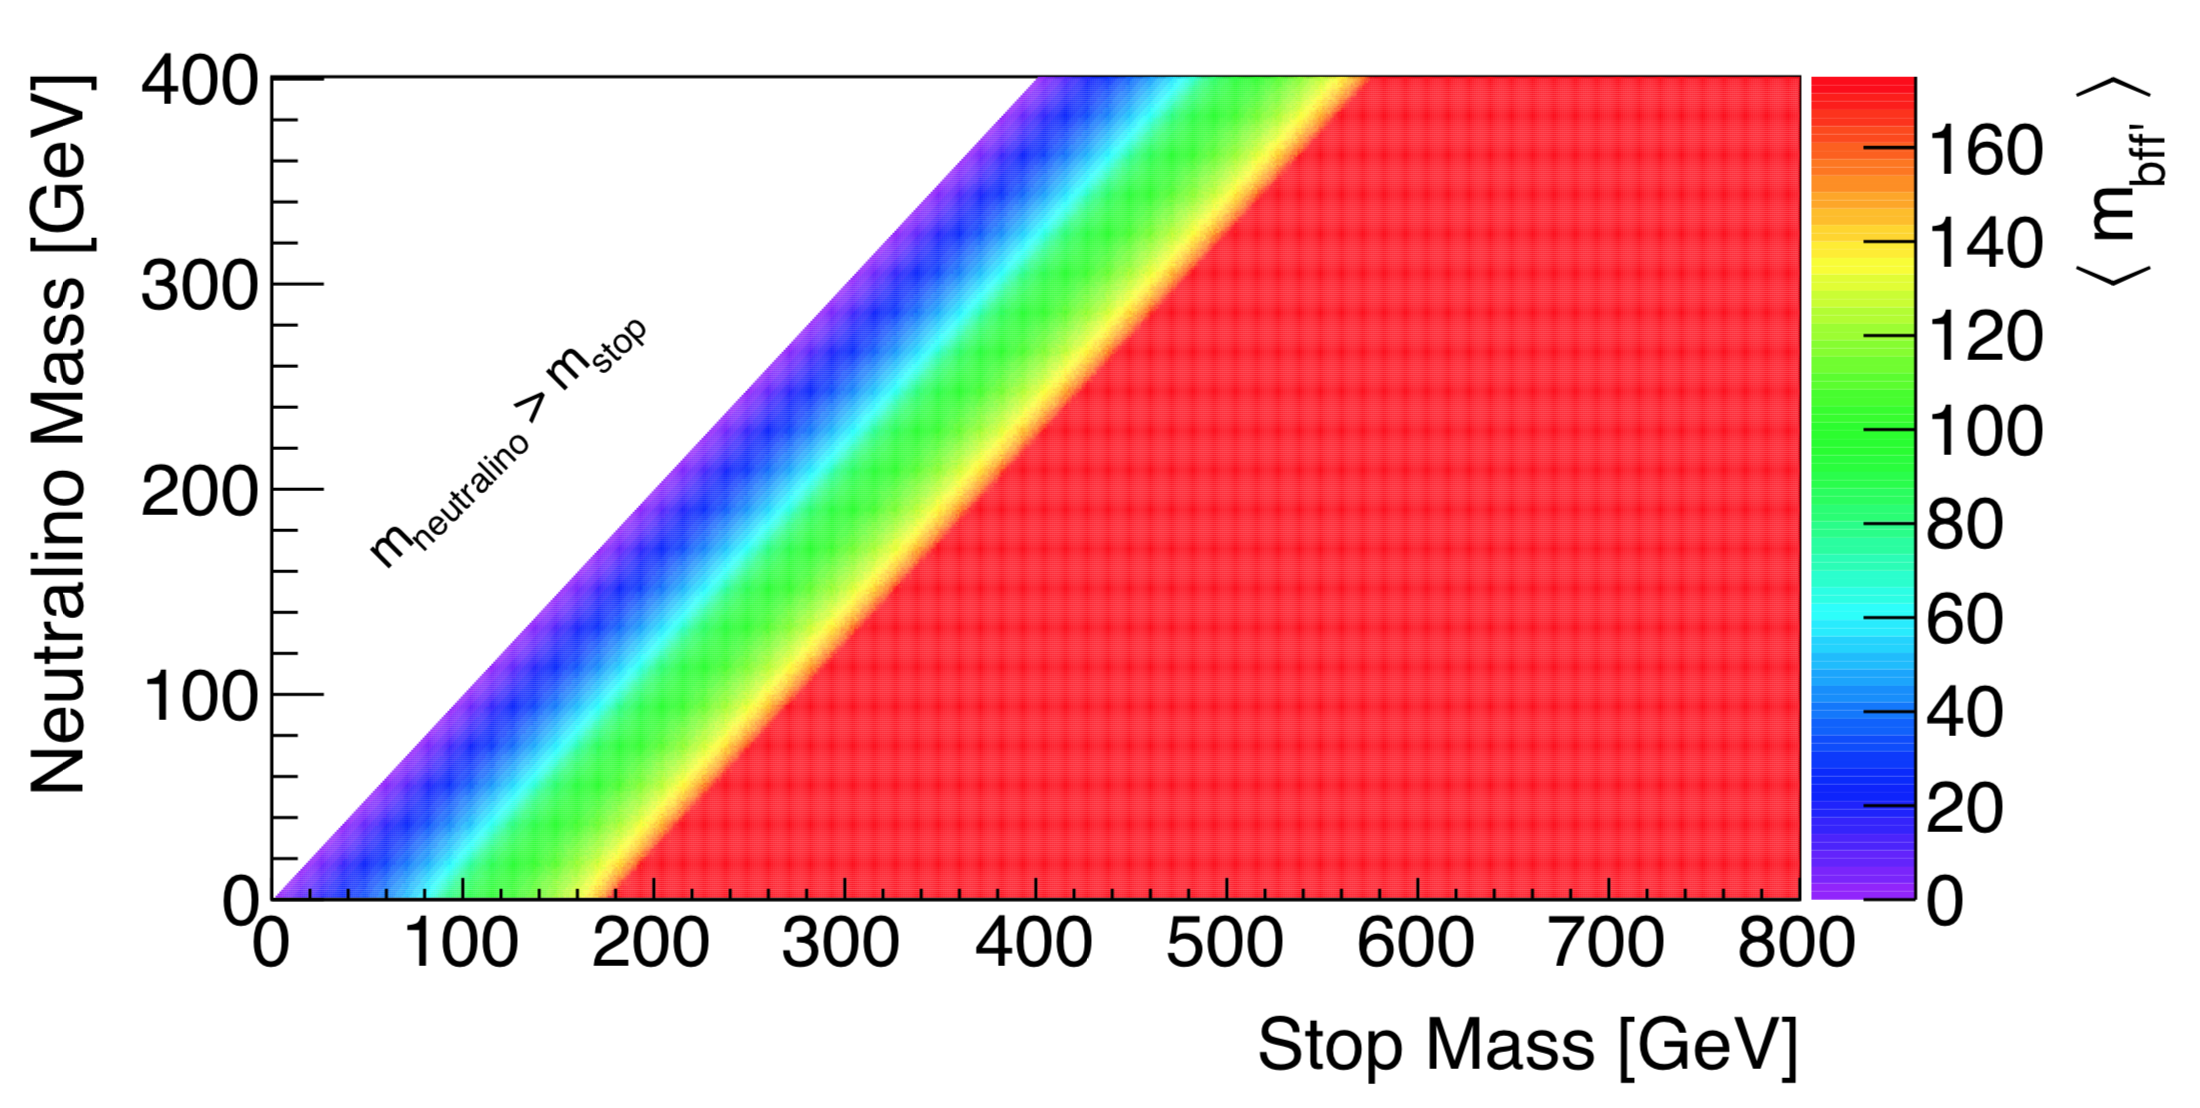
\includegraphics[width=0.75\textwidth]{figures/search_stop2l/nachman_stop_phase_space}
        \caption{
            Average invariant mass of the $b$-quark and SM fermions ($f f^{\prime}$) in the
            final state of the $\stopone \rightarrow b f f^{\prime} \ninoone$ decay, as a function of the mass
            of the \stopone and \ninoone particles.
            Figure taken from Ref.~\cite{Nachman:2016qyc}.
        }
        \label{fig:stop_phase_space}
    \end{center}
\end{figure}

\subsection{Simulation of the Three-body Decay of the Stop}
\label{sec:stop_sim}

% near the boundaries, blah blah blah it is important to get the simulation
% of the spin etc correct ---> MADSPIN

% the effects of stop mixing are particularly exageratted in the regions
% near ∆M = m_top, and so MadSpin...
% these effects are in addition to the kinematic considerations described in the itemized list in the previous section...
% --> THAT IS: PHASE SPACE AND POLARIZATION INFO ACCEPTS THE SIGNAL ACCEPTANCE

\cite{Belanger:2012tm,Perelstein:2008zt,Low:2013aza}

\subsection{Description of the Three-body Decay Final State}
\label{sec:stop_final_state}

% figure stop_phase_space, indicates soft decay products from the stop decays:
%  -> soft b-quarks == stop b-jets, not reconstructuble
%  -> soft W-bosons that are still on-shell --> lepton pT/kinematics similar to that of WW production,
%       especially given that the b-jets are missing for large portions of the three-body phase space
%  -> soft \ninoone == generally low values of the missing transverse moemnetum, as compared to the two-body
%       region, again this makes it more like WW production in the region nearer to the ∆M = m_W diagonal.
